% Aberdeen style guide should be followed when using this
% layout. Their template powerpoint slide is used to extract the
% Aberdeen color and logo but is otherwise ignored (it has little or
% no formatting in it anyway).
%
% http://www.abdn.ac.uk/documents/style-guide.pdf

%%%%%%%%%%%%%%%%%%%% Document Class Settings %%%%%%%%%%%%%%%%%%%%%%%%%
% Pick if you want slides, or draft slides (no animations)
%%%%%%%%%%%%%%%%%%%%%%%%%%%%%%%%%%%%%%%%%%%%%%%%%%%%%%%%%%%%%%%%%%%%%%
%Normal document mode%
\documentclass[10pt,compress]{beamer}
%Draft or handout mode
%\documentclass[10pt,compress,handout]{beamer}
%\documentclass[10pt,compress,handout,ignorenonframetext]{beamer}

%%%%%%%%%%%%%%%%%%%% General Document settings %%%%%%%%%%%%%%%%%%%%%%%
% These settings must be set for each presentation
%%%%%%%%%%%%%%%%%%%%%%%%%%%%%%%%%%%%%%%%%%%%%%%%%%%%%%%%%%%%%%%%%%%%%%
\newcommand{\shortname}{jefferson.gomes@abdn.ac.uk}
\newcommand{\fullname}{Dr Jeff Gomes}
\institute{School of Engineering}
\newcommand{\emailaddress}{}%jefferson.gomes@abdn.ac.uk}
\newcommand{\logoimage}{../../FigBanner/UoAHorizBanner}
\title{Chemical Thermodynamics (EX3029)}
\subtitle{Module 2: Volumetric Properties of Pure Fluids}
\date[ ]{ }

%%%%%%%%%%%%%%%%%%%% Template settings %%%%%%%%%%%%%%%%%%%%%%%%%%%%%%%
% You shouldn't have to change below this line, unless you want to.
%%%%%%%%%%%%%%%%%%%%%%%%%%%%%%%%%%%%%%%%%%%%%%%%%%%%%%%%%%%%%%%%%%%%%%
\usecolortheme{whale}
\useoutertheme{infolines}

% Use the fading effect for items that are covered on the current
% slide.
\beamertemplatetransparentcovered

% We abuse the author command to place all of the slide information on
% the title page.
\author[\shortname]{%
  \fullname\\\ttfamily{\emailaddress}
}


%At the start of every section, put a slide indicating the contents of the current section.
\AtBeginSection[] {
  \begin{frame}
    \frametitle{Section Outline}
    \tableofcontents[currentsection]
  \end{frame}
}

% Allow the inclusion of movies into the Presentation! At present,
% only the Okular program is capable of playing the movies *IN* the
% presentation.
\usepackage{multimedia}
\usepackage{animate}

%% Handsout -- comment out the lines below to create handstout with 4 slides in a page with space for comments
\usepackage{handoutWithNotes}
%\pgfpagesuselayout{2 on 1 with notes}[a4paper,border shrink=10mm]
%%%%% Color settings
\usepackage{color}
%% The background color for code listings (i.e. example programs)
\definecolor{lbcolor}{rgb}{0.9,0.9,0.9}%
\definecolor{UoARed}{rgb}{0.64706, 0.0, 0.12941}
\definecolor{UoALight}{rgb}{0.85, 0.85, 0.85}
\definecolor{UoALighter}{rgb}{0.92, 0.92, 0.92}
\setbeamercolor{structure}{fg=UoARed} % General background and higlight color
\setbeamercolor{frametitle}{bg=black} % General color
\setbeamercolor{frametitle right}{bg=black} % General color
\setbeamercolor{block body}{bg=UoALighter} % For blocks
\setbeamercolor{structure}{bg=UoALight} % For blocks
% Rounded boxes for blocks
\setbeamertemplate{blocks}[rounded]

%%%%% Font settings
% Aberdeen requires the use of Arial in slides. We can use the
% Helvetica font as its widely available like so
% \usepackage{helvet}
% \renewcommand{\familydefault}{\sfdefault}
% But beamer already uses a sans font, so we will stick with that.

% The size of the font used for the code listings.
\newcommand{\goodsize}{\fontsize{6}{7}\selectfont}

% Extra math packages, symbols and colors. If you're using Latex you
% must be using it for formatting the math!
\usepackage{amscd,amssymb} \usepackage{amsfonts}
\usepackage[mathscr]{eucal} \usepackage{mathrsfs}
\usepackage{latexsym} \usepackage{amsmath} \usepackage{bm}
\usepackage{amsthm} \usepackage{textcomp} \usepackage{eurosym}
% This package provides \cancel{a} and \cancelto{a}{b} to "cancel"
% expressions in math.
\usepackage{cancel}

\usepackage{comment} 

%% Handsout -- comment out the lines below to create handstout with 4 slides in a page with space for comments
\usepackage{handoutWithNotes}

\mode<handout>
{
\usepackage{pgf,pgfpages}

\pgfpagesdeclarelayout{2 on 1 boxed with notes}
{
\edef\pgfpageoptionheight{\the\paperheight} 
\edef\pgfpageoptionwidth{\the\paperwidth}
\edef\pgfpageoptionborder{0pt}
}
{
\setkeys{pgfpagesuselayoutoption}{landscape}
\pgfpagesphysicalpageoptions
    {%
        logical pages=4,%
        physical height=\pgfpageoptionheight,%
        physical width=\pgfpageoptionwidth,%
        last logical shipout=2%
    } 
\pgfpageslogicalpageoptions{1}
    {%
    border code=\pgfsetlinewidth{1pt}\pgfstroke,%
    scale=1,
    center=\pgfpoint{.25\pgfphysicalwidth}{.75\pgfphysicalheight}%
    }%
\pgfpageslogicalpageoptions{2}
    {%
    border code=\pgfsetlinewidth{1pt}\pgfstroke,%
    scale=1,
    center=\pgfpoint{.25\pgfphysicalwidth}{.25\pgfphysicalheight}%
    }%
\pgfpageslogicalpageoptions{3}
    {%
    border shrink=\pgfpageoptionborder,%
    resized width=.7\pgfphysicalwidth,%
    resized height=.5\pgfphysicalheight,%
    center=\pgfpoint{.75\pgfphysicalwidth}{.29\pgfphysicalheight},%
    copy from=3
    }%
\pgfpageslogicalpageoptions{4}
    {%
    border shrink=\pgfpageoptionborder,%
    resized width=.7\pgfphysicalwidth,%
    resized height=.5\pgfphysicalheight,%
    center=\pgfpoint{.75\pgfphysicalwidth}{.79\pgfphysicalheight},%
    copy from=4
    }%

\AtBeginDocument
    {
    \newbox\notesbox
    \setbox\notesbox=\vbox
        {
            \hsize=\paperwidth
            \vskip-1in\hskip-1in\vbox
            {
                \vskip1cm
                Notes\vskip1cm
                        \hrule width\paperwidth\vskip1cm
                    \hrule width\paperwidth\vskip1cm
                        \hrule width\paperwidth\vskip1cm
                    \hrule width\paperwidth\vskip1cm
                        \hrule width\paperwidth\vskip1cm
                    \hrule width\paperwidth\vskip1cm
                    \hrule width\paperwidth\vskip1cm
                    \hrule width\paperwidth\vskip1cm
                        \hrule width\paperwidth
            }
        }
        \pgfpagesshipoutlogicalpage{3}\copy\notesbox
        \pgfpagesshipoutlogicalpage{4}\copy\notesbox
    }
}
}

%\pgfpagesuselayout{2 on 1 boxed with notes}[letterpaper,border shrink=5mm]
%\pgfpagesuselayout{2 on 1 boxed with notes}[letterpaper,border shrink=5mm]


% Get rid of font warnings as modern LaTaX installations have scalable
% fonts
\usepackage{type1cm} 

%\usepackage{enumitem} % continuous numbering throughout enumerate commands

% For exact placement of images/text on the cover page
\usepackage[absolute]{textpos}
\setlength{\TPHorizModule}{1mm}%sets the textpos unit
\setlength{\TPVertModule}{\TPHorizModule} 

% Source code formatting package
\usepackage{listings}%
\lstset{ backgroundcolor=\color{lbcolor}, tabsize=4,
  numberstyle=\tiny, rulecolor=, language=C++, basicstyle=\goodsize,
  upquote=true, aboveskip={1.5\baselineskip}, columns=fixed,
  showstringspaces=false, extendedchars=true, breaklines=false,
  prebreak = \raisebox{0ex}[0ex][0ex]{\ensuremath{\hookleftarrow}},
  frame=single, showtabs=false, showspaces=false,
  showstringspaces=false, identifierstyle=\ttfamily,
  keywordstyle=\color[rgb]{0,0,1},
  commentstyle=\color[rgb]{0.133,0.545,0.133},
  stringstyle=\color[rgb]{0.627,0.126,0.941}}

% Allows the inclusion of other PDF's into the final PDF. Great for
% attaching tutorial sheets etc.
\usepackage{pdfpages}
\setbeamercolor{background canvas}{bg=}  

% Remove foot note horizontal rules, they occupy too much space on the slide
\renewcommand{\footnoterule}{}

% Force the driver to fix the colors on PDF's which include mixed
% colorspaces and transparency.
\pdfpageattr {/Group << /S /Transparency /I true /CS /DeviceRGB>>}

% Include a graphics, reserve space for it but
% show it on the next frame.
% Parameters:
% #1 Which slide you want it on
% #2 Previous slides
% #3 Options to \includegraphics (optional)
% #4 Name of graphic
\newcommand{\reserveandshow}[4]{%
\phantom{\includegraphics<#2|handout:0>[#3]{#4}}%
\includegraphics<#1>[#3]{#4}%
}

\newcommand{\frc}{\displaystyle\frac}
\newcommand{\red}{\textcolor{red}}
\newcommand{\blue}{\textcolor{blue}}
\newcommand{\green}{\textcolor{green}}
\newcommand{\purple}{\textcolor{purple}}
 
\begin{document}

% Title page layout
\begin{frame}
  \titlepage
  \vfill%
  \begin{center}
    \includegraphics[clip,width=0.8\textwidth]{\logoimage}
  \end{center}
\end{frame}

% Table of contents
\frame{ \frametitle{Slides Outline}
  \tableofcontents
}


%%%%%%%%%%%%%%%%%%%% The Presentation Proper %%%%%%%%%%%%%%%%%%%%%%%%%
% Fill below this line with \begin{frame} commands! It's best to
% always add the fragile option incase you're going to use the
% verbatim environment.
%%%%%%%%%%%%%%%%%%%%%%%%%%%%%%%%%%%%%%%%%%%%%%%%%%%%%%%%%%%%%%%%%%%%%%


%%%
%%% SECTION
%%%
\section{General Remarks}

%%%
%%% Slides
%%%
\begin{frame}
 \frametitle{Aims and Objectives}
   \begin{enumerate}
     \item<1-> In Module 1, we learnt:
       \begin{enumerate}
         \item<1-> the laws of Thermodynamics and how they describe thermal equilibrium of species in closed and opened systems.
         \item<1-> how to obtain and calculate relevant thermodynamics properties for chemical species.
         \item<1-> reversibility  of processes.
       \end{enumerate} 
     \item<2-> This Module focuses on 
         \begin{enumerate}
           \item<2-> PVT behaviour of pure chemical species in equilibrium,
           \item<2-> Equations of state commonly used in industry.
         \end{enumerate}
   \end{enumerate}

\end{frame}


%%%
%%% SECTION
%%%
\section{Bibliography}
\begin{frame}
 \frametitle{Suggested References}
  Literature relevant for this module:
  \begin{enumerate}[(a)]
   \item J.M. Smith, H.C. Van Ness, M.M. Abbott, $\lq$Introduction to Chemical Engineering Thermodynamics', 6$^{th}$ Edition: Chapter 3;
   \item Y.A. Cengel, M.A. Boles, $\lq$Thermodynamics -- An Engineering Approach', 5$^{th}$ Edition: Chapter 3; 
   \item M.J. Moran, H.N. Saphiro, D.D. Boettner, M.B. Bailey, $\lq$Principles of Engineering Thermodynamics', 7$^{th}$ Edition: Chapters 3;
   \item C. Borgnakke, R.E. Sonntag,$\lq$Fundamentals of Thermodynamics',8$^{th}$ Edition: Chapter 2.
  \end{enumerate}
\end{frame}



%%%
%%% SECTION
%%%
\section{PVT Behaviour of Pure Substances}

%%%
%%% SUBSECTION
%%%
\subsection{Phase Diagram and Gibbs Rule} 

%%%
%%% Slide
%%%
\scriptsize
\begin{frame}
 \frametitle{PT Diagram for Pure Substances}
  \begin{columns}
    \begin{column}[l]{0.5\linewidth}\scriptsize
      \begin{enumerate}[(a)]%\scriptsize
        \item <1-> Recall the Gibbs phase rule (Module 1):
           \visible<1->{\begin{displaymath}
             \Psi = 2 + \mathcal{C} - \mathcal{P}
           \end{displaymath}
             where $\Psi$ is the number of \textcolor{blue}{degrees of freedom} for the system, \textcolor{blue}{2} refers to the independent variables ($T$ and $P$), \textcolor{blue}{$\mathcal{C}$} is the number of chemical species and \textcolor{blue}{$\mathcal{P}$} is the number of phases;}   
        \item<2-> The \textcolor{blue}{$PT$ phase diagram} describes fluid behaviour and phase change; 
        \item<3-> For example: \textcolor{blue}{A}-\;-\;-\textcolor{red}{B} defines a phase transition from \textcolor{blue}{liquid} to \textcolor{red}{gas} regions without crossing the phase boundary (vaporisation);
        \item<4-> \textcolor{red}{However}, there is \textcolor{blue}{no} information about the volume in the {\it PT} diagram.
      \end{enumerate}
    \end{column}
    \begin{column}[l]{0.5\linewidth}\scriptsize
      \begin{figure}%
        \begin{center}
          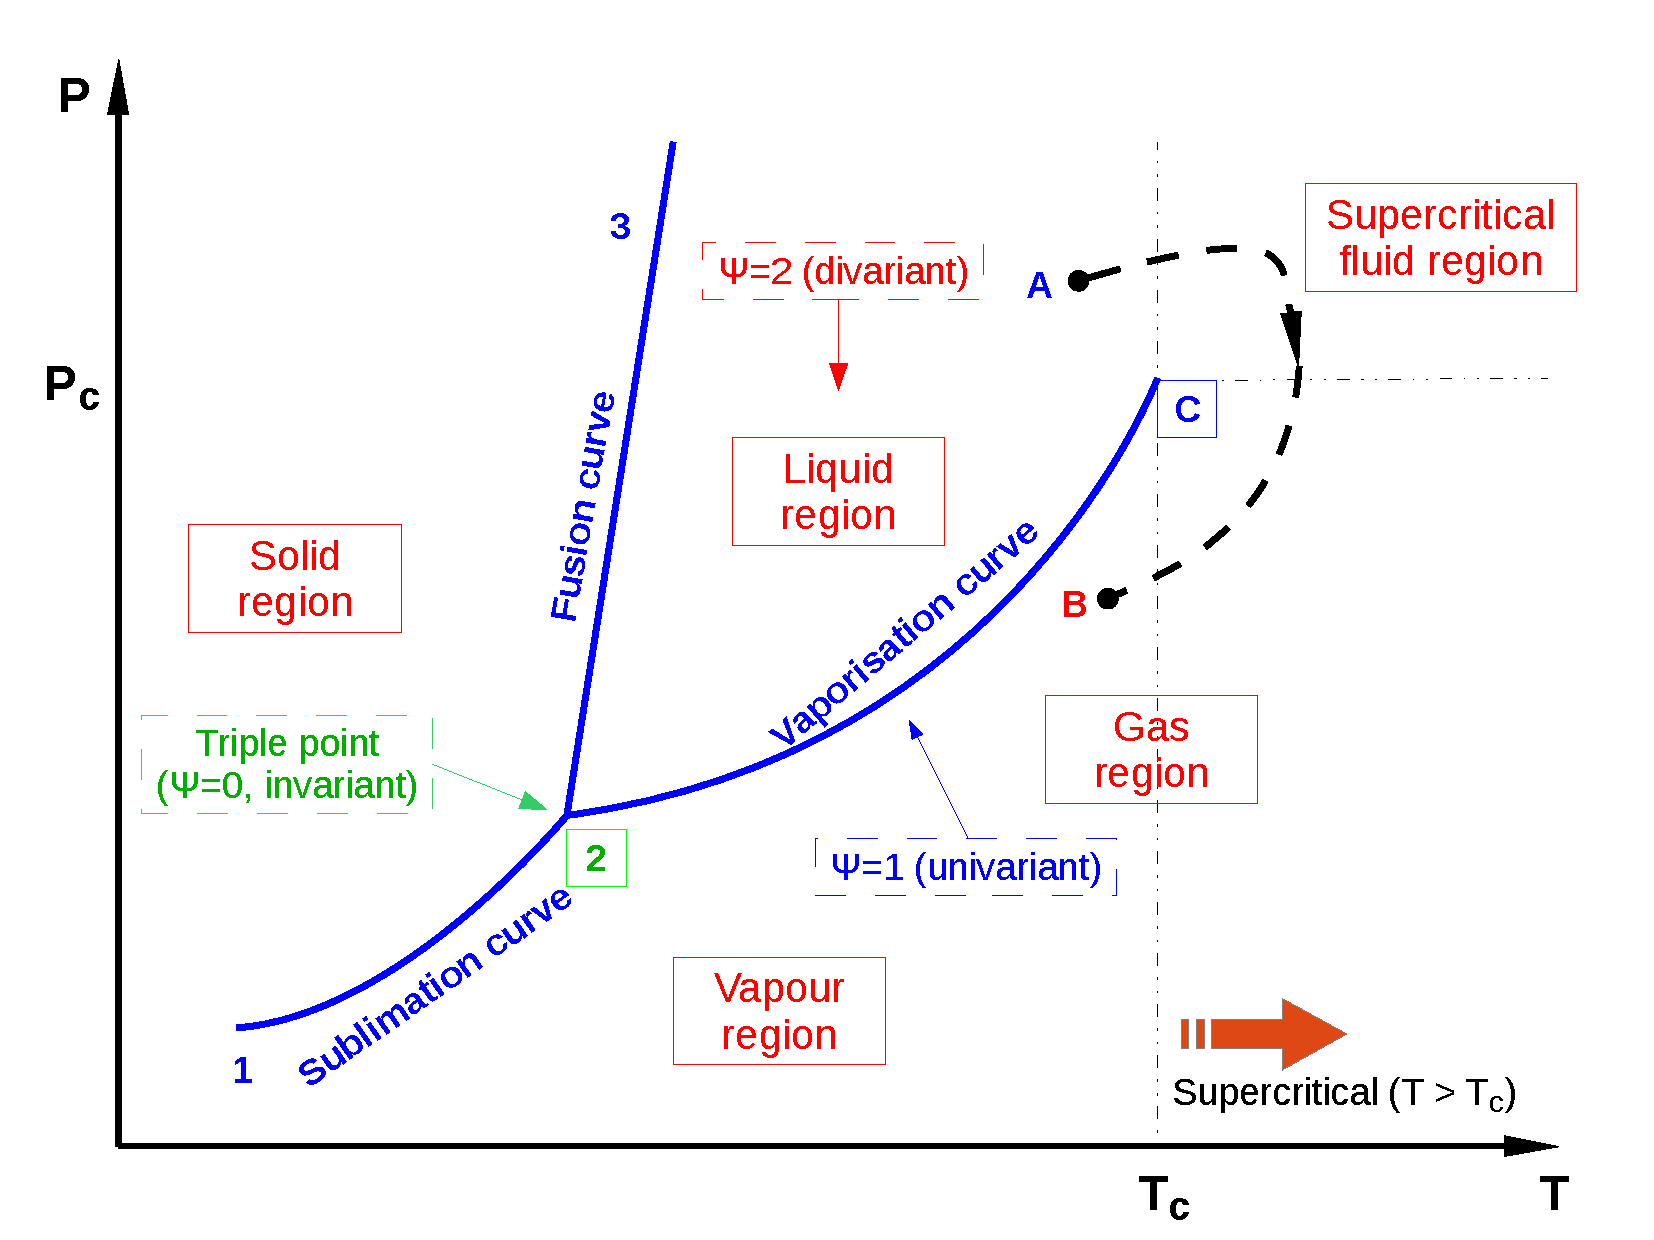
\includegraphics[width=1.05\columnwidth,clip]{./../Pics/PT_Diagram}
        \end{center}
      \end{figure}
    \end{column}
  \end{columns}
\end{frame}
\normalsize



%%%
%%% Slide
%%%
\scriptsize
\begin{frame}
 \frametitle{PV Diagram}
  \begin{columns}
    \begin{column}[l]{0.5\linewidth}
      \visible<1->{\begin{figure}%
        \begin{center}
          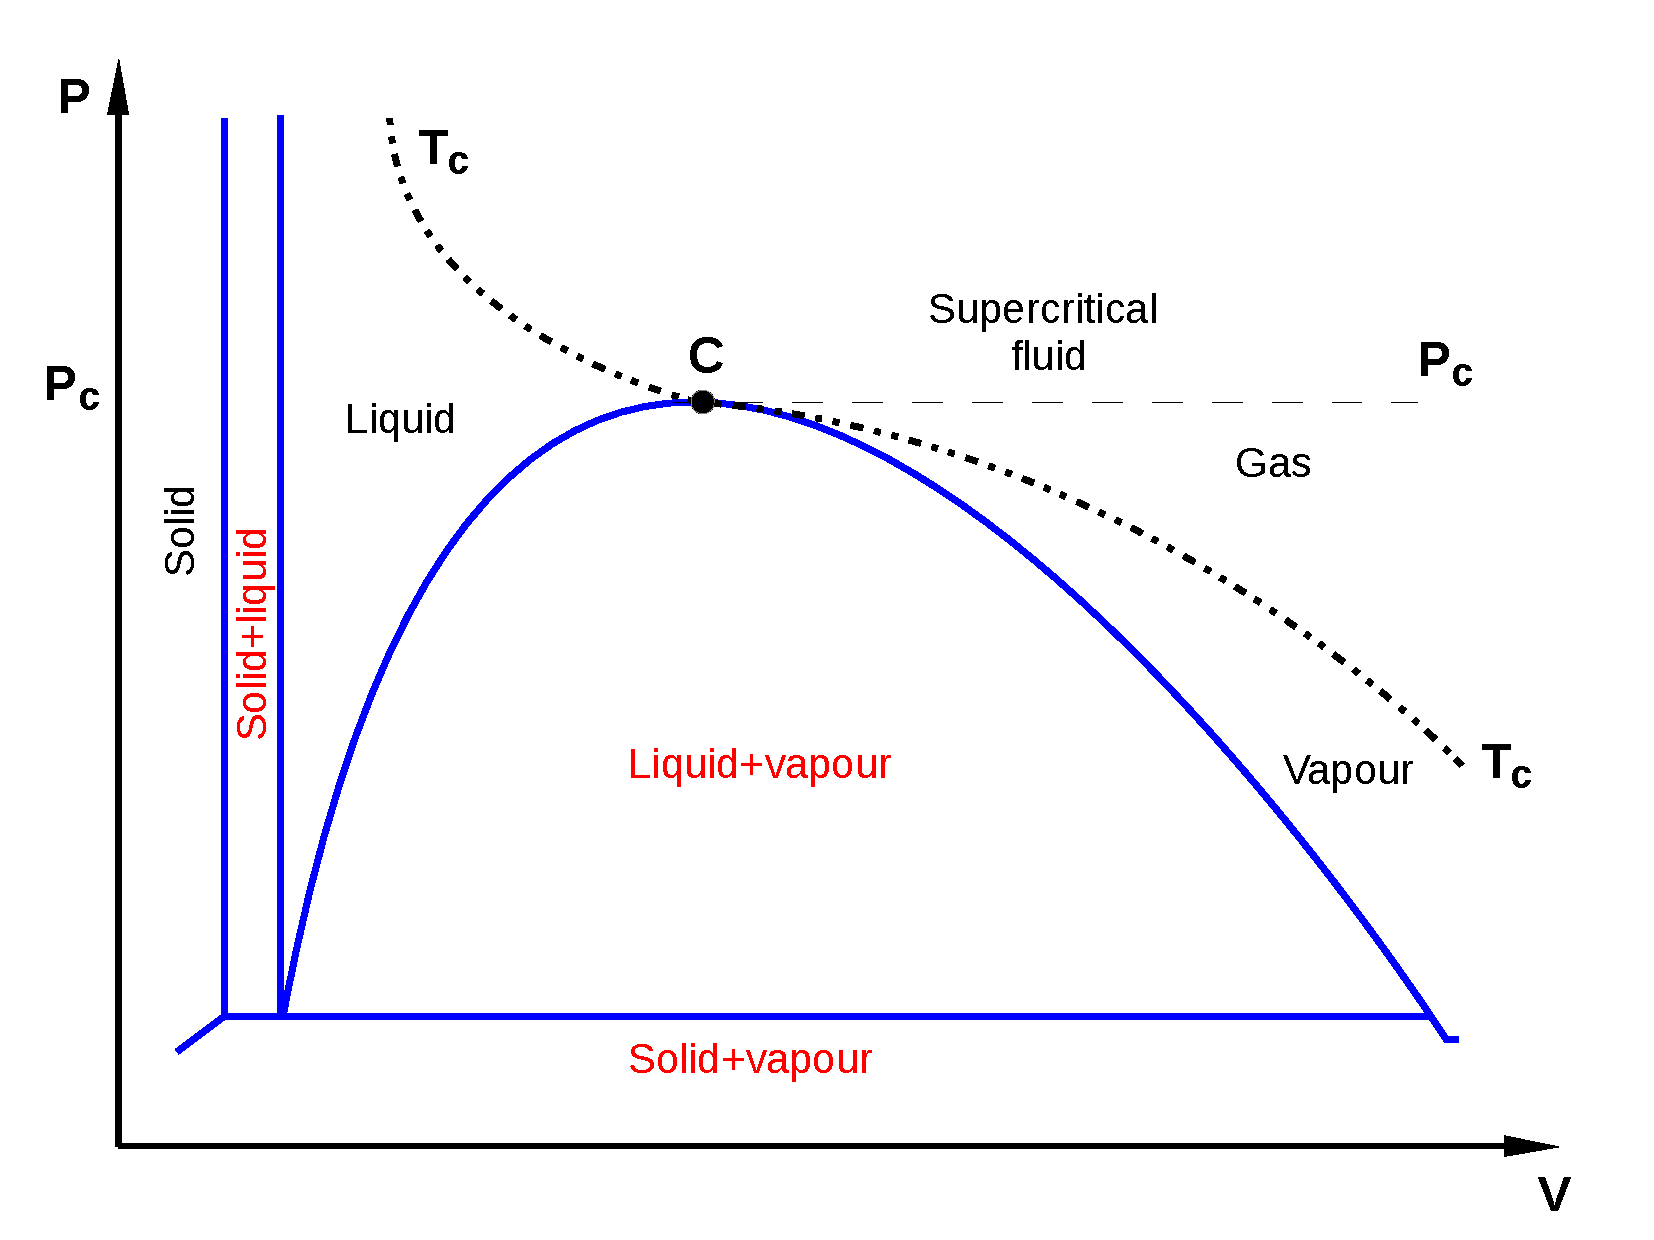
\includegraphics[width=\columnwidth,clip]{./../Pics/PV_Diagram1}
        \end{center}
      \end{figure}}
      \begin{enumerate} \scriptsize
        \item<1-> Two-phase regions (e.g., liquid+vapor) are represented by \textcolor{red}{areas} and;
        \item<2-> Lines represent the actual transition transition between \textcolor{blue}{single phase} to \textcolor{blue}{two phases} regions, thus;
        \item<2-> The \textcolor{blue}{triple point} is the horizontal line between the 3 phases;
      \end{enumerate}
    \end{column}
    \begin{column}[l]{0.5\linewidth}\scriptsize
      \visible<3->{\begin{figure}%
        \begin{center}
          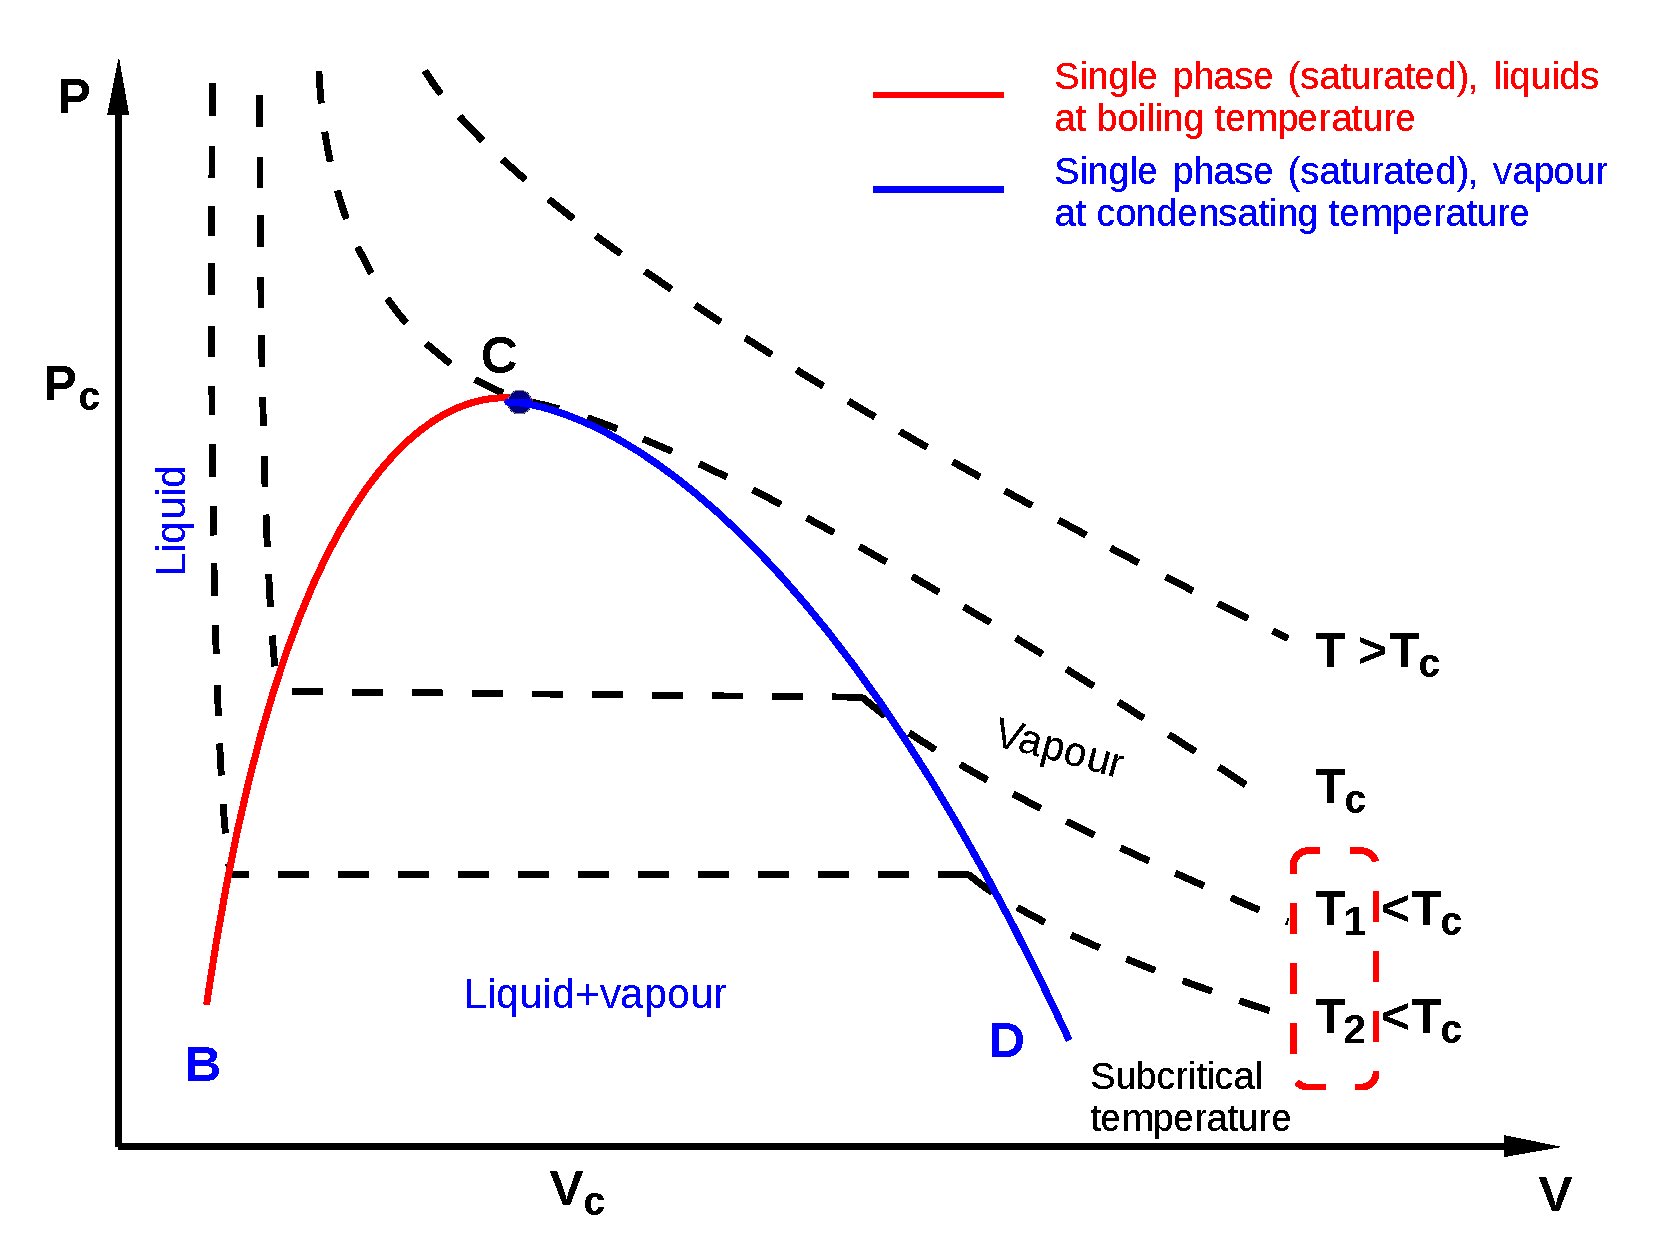
\includegraphics[width=\columnwidth,clip]{./../Pics/PV_Diagram2}
        \end{center}
      \end{figure}}
      \begin{enumerate}\setcounter{enumi}{3}
        \item<3-> The isotherms range from \textcolor{blue}{subcooled liquid} to \textcolor{blue}{superheated vapor} regions; 
        \item<3-> Isotherms are \textcolor{red}{steep} in the \textcolor{blue}{subcooled liquid}  region because liquid volumes have little changes with large change in pressure.
      \end{enumerate}
    \end{column}
  \end{columns}
\end{frame}
\normalsize

%%%
%%% Slide
%%%
\scriptsize
\begin{frame}
 \frametitle{PV Diagram}
      \visible<1->{\begin{figure}%
        \begin{center}
          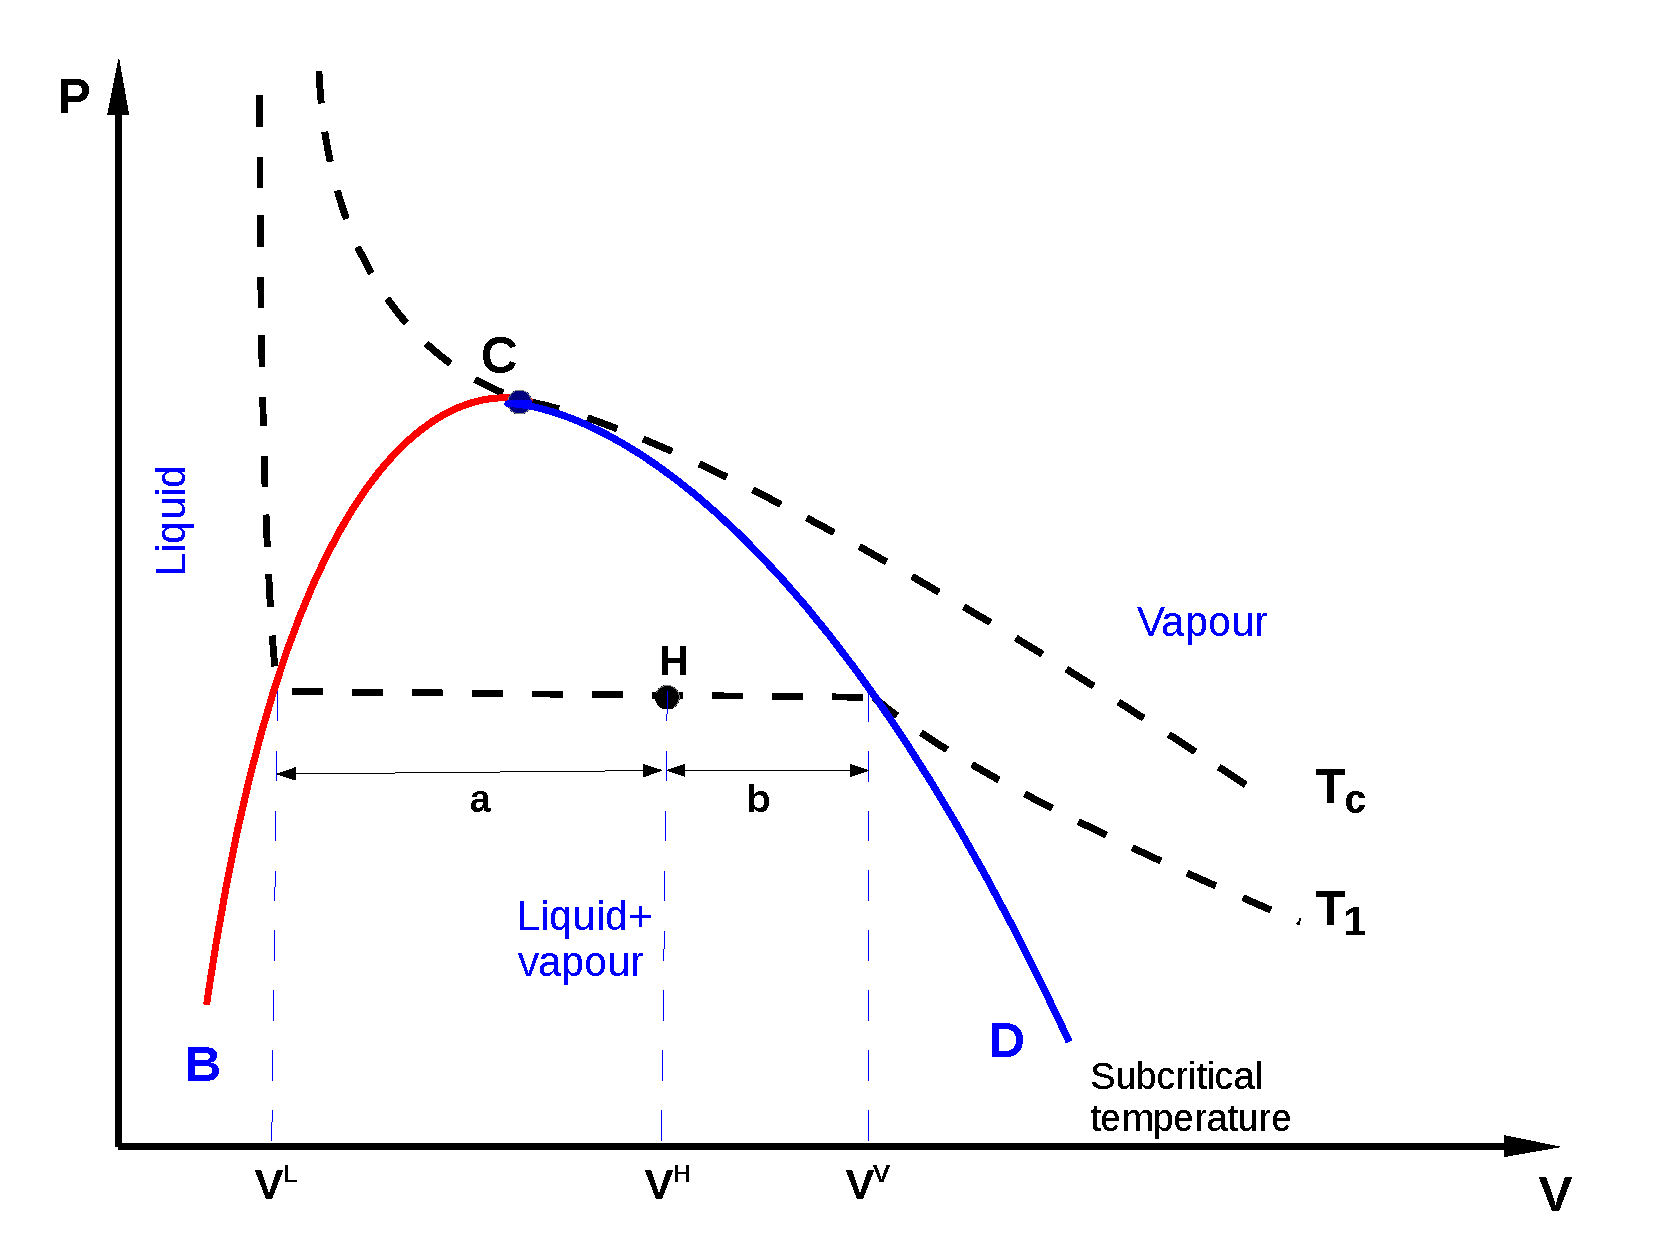
\includegraphics[width=.6\columnwidth,clip]{./../Pics/PV_Diagram3}
        \end{center}
      \end{figure}}
      \visible<2->{\begin{displaymath}
         \frc{a}{b} = \frc{V^{H}-V^{L}}{V^{V}-V^{H}} = \frc{m^{V}}{m^{L}} = \frc{\text{mass of saturated vapour}}{\text{mass of saturated liquid}}
      \end{displaymath}}
     
\end{frame}
\normalsize

%%%
%%% Slide
%%%
\scriptsize
\begin{frame}
 \frametitle{Single Phase region}
    \begin{enumerate}\scriptsize
      \item<1-> \textcolor{blue}{Equations of State (EOS)} relates pressure, molar or specific volume and temperature of any \textcolor{blue}{pure homogeneous fluid} in equilibrium states;
      \item<2-> We can express it as a general functional,
          \visible<2->{\begin{displaymath}
              f\left(P, V, T\right) = 0
          \end{displaymath} 
          where $P$, $V$ or $T$ can be expressed as a function of two of this properties.}
      \item<3-> For example, we can represent the volume as $V=V\left(T,P\right)$, thus
          \visible<3->{\begin{equation}
              dV = \left(\frc{\partial V}{\partial T}\right)_{P} dT + \left(\frc{\partial V}{\partial P}\right)_{T} dP \;\;\Longrightarrow \;\; \textcolor{blue}{\frc{dV}{V} = \beta dT - \kappa dP} \label{genericV}
          \end{equation} 
            with $\beta  =  \frc{1}{V}\left(\frc{\partial V}{\partial T}\right)_{P}$ (volume expansivity) and $\kappa = -\frc{1}{V}\left(\frc{\partial V}{\partial P}\right)_{T}$ (isothermal compressibility).
           }
      \item<4-> A few useful remarks:
        \begin{itemize}\scriptsize
          \item<4-> For \textcolor{blue}{incompressible fluids}: $\beta$ and $\kappa$ are zero;
          \item<4-> For liquids: $\beta>0$ (except for liquid H$_{2}$O at $0\leq T\leq 4^{\circ}$C) and $\kappa>0$  
        \end{itemize}
      \item<5-> Close to the critical point, $\beta$ and $\kappa$ are assumed constant, thus \blue{Eqn.~\ref{genericV}} becomes, 
        \visible<5->{\begin{displaymath}
            \ln\frc{V_{2}}{V_{1}} = \beta\left(T_{2}-T_{1}\right) - \kappa\left(P_{2}-P_{1}\right)
        \end{displaymath}}
    
    \end{enumerate}
\end{frame}
\normalsize

%%%
%%% SECTION
%%%
\section{Equations of State (EOS)}

%%%
%%% Slide
%%%
\scriptsize
\begin{frame}
 \frametitle{Summary List of EOS}
      \visible<1->{\begin{figure}%
        \begin{center}
          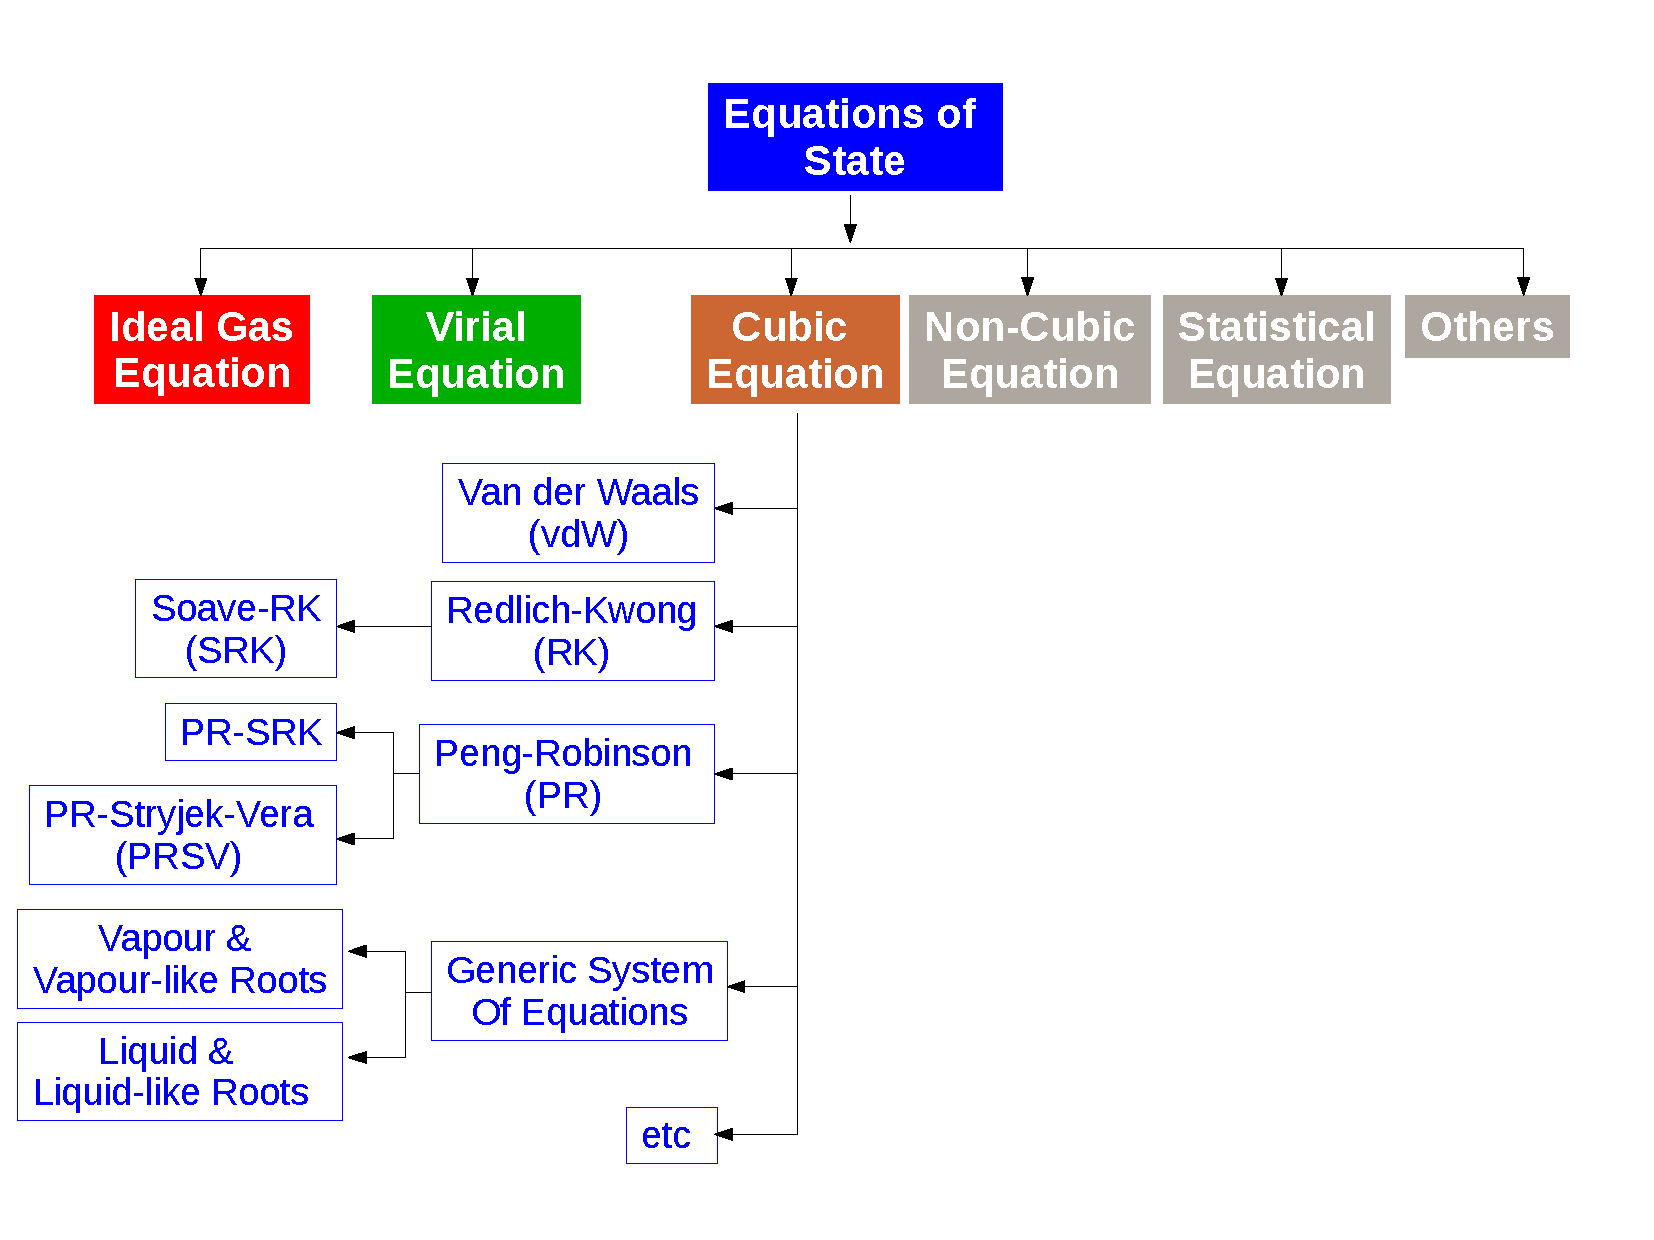
\includegraphics[width=0.9\columnwidth,clip]{./../Pics/ListEOS}
        \end{center}
      \end{figure}}
\end{frame}
\normalsize


%%%
%%% SUBSECTION
%%%
\subsection{Virial EOS}

%%%
%%% Slide
%%%
\scriptsize
\begin{frame}
 \frametitle{Virial Expansion}
   \begin{columns}
    \begin{column}[l]{0.5\linewidth}
      \begin{enumerate} \scriptsize
        \item<1-> $\left(PV\right)$ along an isotherm can be expressed as function of {\bf P} by a \textcolor{blue}{power series},
           \visible<1->{\begin{displaymath}
             \left(PV\right) = a + bP + cP^{2} + dP^{3} + \cdots
           \end{displaymath}}
        \item<2-> Defining $b=aB^{\prime}$, $c=aC^{\prime}$, $d=aD^{\prime}$, $\cdots$, then
           \visible<2->{\begin{equation}\label{Mod3:VirialEoS1}
             \left(PV\right) = a\left( 1 + B^{\prime}P + C^{\prime}P^{2} + D^{\prime}P^{3} + \cdots\right) 
           \end{equation}}
        \item<2-> $B^{\prime}$, $C^{\prime}$ and $D^{\prime}$ are constants, characteristic for each chemical species and temperature-dependent $\left(\text{i.e.,} B^{\prime}=B^{\prime}(T), C^{\prime}=C^{\prime}(T)\right)$  
        \item<3-> In the limit case -- $P\rightarrow 0$, \textcolor{blue}{$\left(PV\right)$ for all gases}:\\
           \begin{displaymath}
              \visible<3->{\textcolor{blue}{\left(PV\right)^{\star} =}} 
                   \begin{cases}
                      \visible<3->{a = f\left(T\right)} \\
                      \visible<4->{\textcolor{blue}{a= RT}}\\ 
                   \end{cases}
           \end{displaymath}
           \visible<4->{where $R$ is a proportionally constant, i.e.,  universal gas constant.}
        \item<5-> At this limiting case, $\left(PV\right)_{T}^{\star} = R \times 273.16$. 
      \end{enumerate}
    \end{column}
    \begin{column}[l]{0.5\linewidth}\scriptsize
     \begin{enumerate}\setcounter{enumi}{5}
       \item<6->For \textcolor{blue}{ideal gasses}, pressure is sufficiently small $\left(P\rightarrow 0\right)$. 
       \item<6-> This means that the molecules are separated by infinite distances, and therefore the \textcolor{blue}{intermolecular forces approaches zero}. 
     \end{enumerate}
      \visible<3->{\begin{figure}%
        \begin{center}
          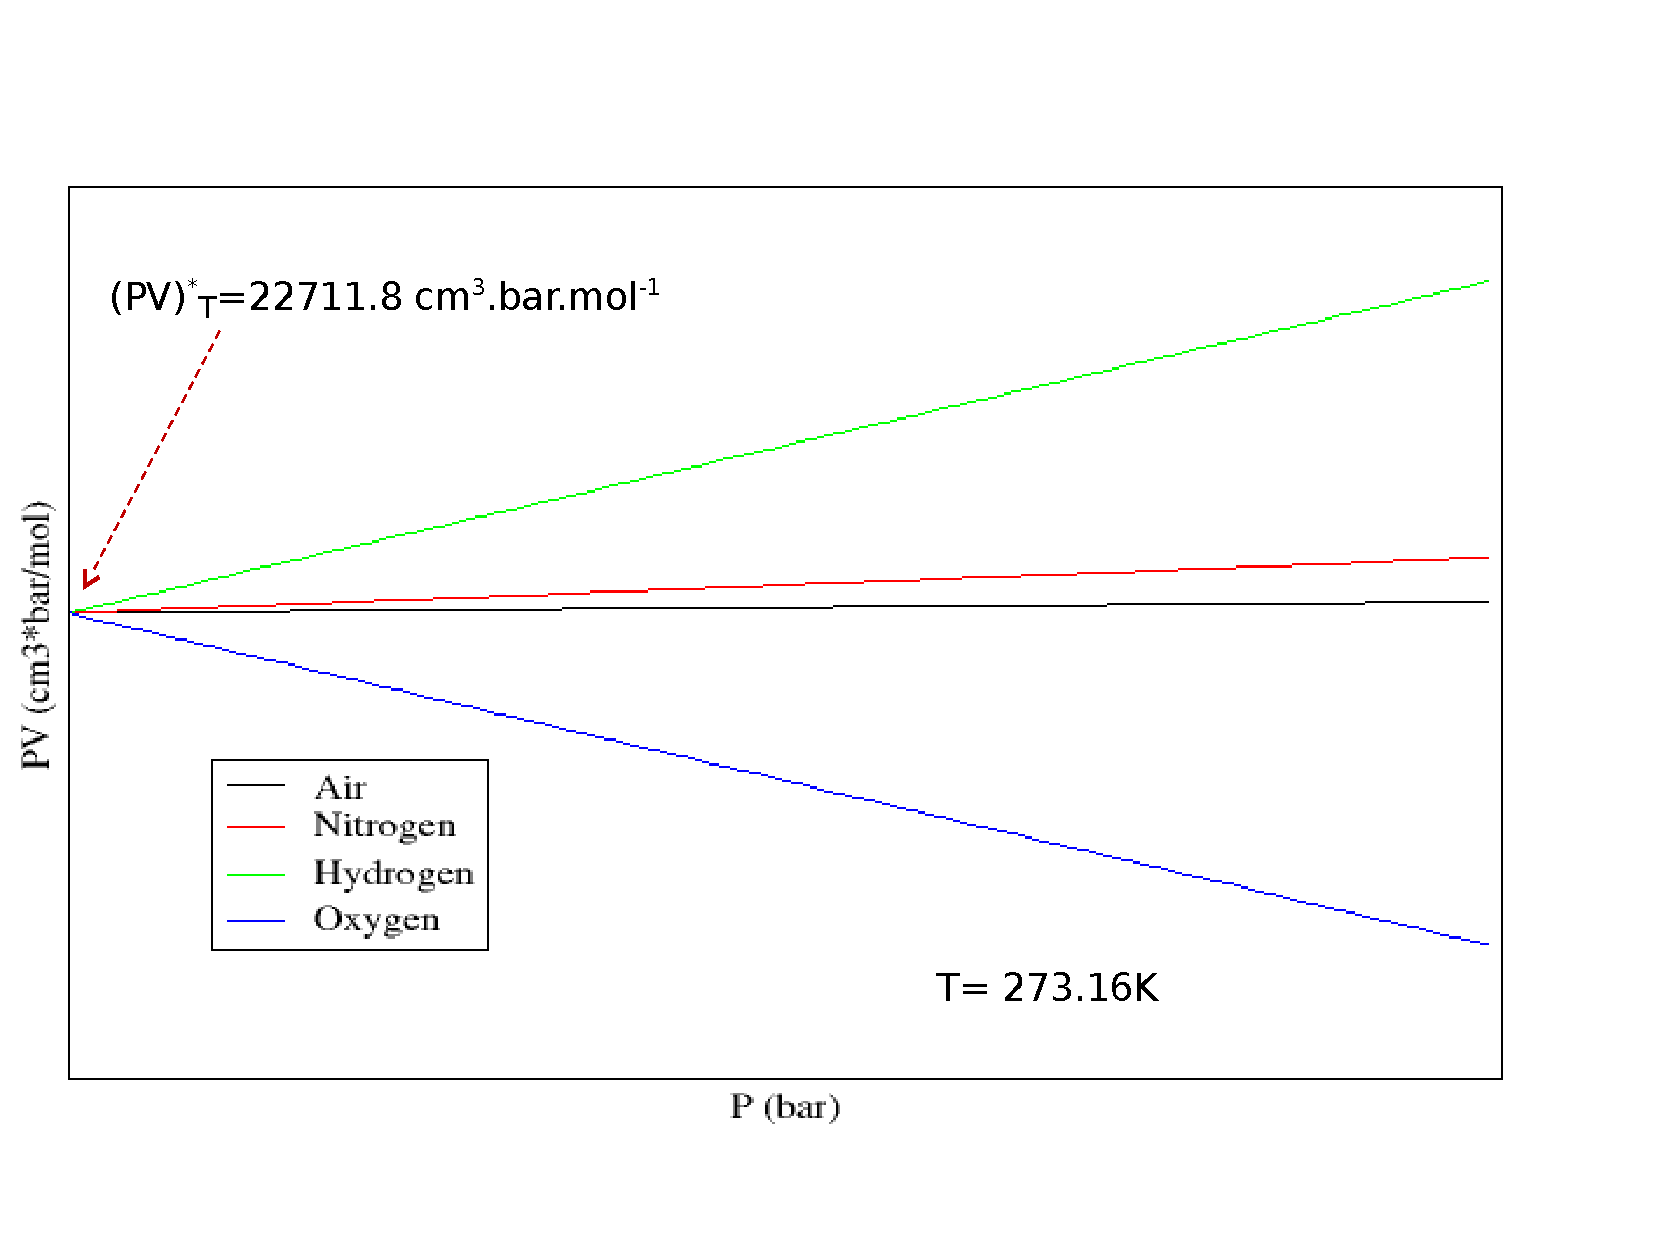
\includegraphics[width=1.05\columnwidth,clip]{./../Pics/Virial_EOS}
        \end{center}
      \end{figure}}
    \end{column}
  \end{columns}

\end{frame}
\normalsize


%%%
%%% Slide
%%%
\scriptsize
\begin{frame}
 \frametitle{Compressibility Factor -- $Z$}
   \begin{enumerate}\setcounter{enumi}{7}\scriptsize
     \item<1-> The {\it Virial expansion} is considered the only EOS based on rigorous mathematical derivation. It can also be derived from statistical mechanics leading to physical  significance of the virial coefficients;
     \item<2->The original form of the Virial EOS (Eqn.~\ref{Mod3:VirialEoS1}) can be rewritten as
        \begin{equation}\label{Mod3:VirialEoS2}
            \visible<2->{\frc{PV}{RT}} \visible<3->{ = \textcolor{red}{Z}} = \visible<2->{1 + B^{\prime}P + C^{\prime}P^{2} + D^{\prime}P^{3} + \cdots}
        \end{equation}
     \item<4-> \textcolor{red}{$Z$} is the \textcolor{blue}{compressibility factor} and is commonly used to estimate the deviation from ideal gas behaviour.
     \item<5->Therefore, the Virial EOS can be represented by 2 main forms:
        \begin{equation}
          Z = \frc{PV}{RT} =
             \begin{cases}
                1 + \textcolor{blue}{\frc{B}{V}} + \textcolor{red}{\frc{C}{V^{2}}} + \textcolor{purple}{\frc{D}{V^{3}}} + \cdots \\
                \visible<6->{1 + \blue{B^{\prime}P} + \red{C^{\prime}P^{2}} + \purple{D^{\prime}P^{3}} + \cdots} \\
                \visible<7->{1 + \blue{\frc{B}{RT}P} + \red{\frc{C-B^{2}}{\left(RT\right)^{2}}P^{2}} + \purple{\frc{D-3BC+2B^{2}}{\left(RT\right)^{3}}P^{3}} + \cdots}
             \end{cases}
        \end{equation}
     \item<8-> Thus, for real cases
        \begin{equation}
          \visible<8->{Z = \frc{PV}{RT} =}
             \begin{cases}
                \visible<8->{1 + \blue{B^{\prime}P} = 1 + \blue{\frc{BP}{RT}} \hspace{2.6cm} \Rightarrow\;\; \text{Low-Moderate pressures -- P}<\text{15 bar}}\\
                \visible<9->{1 + \blue{B^{\prime}P} + \red{C^{\prime}P^{2}}  = 1 + \blue{\frc{BP}{RT}} + \red{\frc{C-B^{2}}{\left(RT\right)^{2}}P^{2}}\;\;\Rightarrow\;\; \text{High pressures \red{but} below the } P_{c}}
             \end{cases}
        \end{equation}
             
   \end{enumerate}
\end{frame}
\normalsize


%%%
%%% SUBSECTION
%%%
\subsection{Cubic EOS}

%%%
%%% Slide
%%%
\scriptsize
\begin{frame}
 \frametitle{Generic Cubic EOS}
    \begin{enumerate}\scriptsize
      \item<1-> The simplest equations able to represent both \blue{liquid} and \blue{vapour} phases behaviour but \red{not} for two-phase condition;
      \item<2-> They are designed to be used in a wide range of temperature and pressure;
      \item<3-> General format of a cubic equation on $V$,
         \begin{equation}\label{Mod3:GenCubicEqn}
            \visible<3->{
             P = \frc{RT}{V-b} - \frc{\theta\left(V-\eta\right)}{\left(V-b\right)\left(V^{2}+\kappa V + \lambda\right)}
            }
         \end{equation}
         \visible<3->{Where $b$, $\theta$, $\kappa$, $\lambda$ and $\eta$ are parameters that depend on \blue{T} and \blue{composition} (for mixtures).}
      \item<4-> If $\eta=b$, $\theta=a(T)$,$\kappa=\left(\epsilon+\sigma\right)b$ and $\lambda=\epsilon\sigma b^{2}$, we can define a generic cubic equation of state,
           \visible<4->{\begin{equation}\label{Mod3:GenCubicEOS}
              P = \frc{RT}{V-b} - \frc{a(T)}{\left(V-\epsilon b\right)\left(V+\sigma b\right)}
           \end{equation}
           where $\epsilon$ and $\sigma$ are constants.}
       \item<5-> $a(T)$ and $b$ are specific for chemical species and defined as,
           \visible<5->{\begin{displaymath} 
             a(T) = \Psi\frc{\alpha(T)R^{2}T_{c}^{2}}{P_{c}}\;\;\;\text{ and }\;\;\; b=\Omega\frc{R T_{c}}{P_{c}}
           \end{displaymath}
           $\Psi$ and $\Omega$ are constants and may vary for different cubic EOS.} 
    \end{enumerate}
\end{frame}
\normalsize

%%%
%%% Slide
%%%
\scriptsize
\begin{frame}
 \frametitle{Cubic Equations of State}
    \visible<1->{\begin{block}{van der Waals}
        If we set $\eta=b$, $\theta=a$ and $\kappa=\lambda=0$, Eqn.~\ref{Mod3:GenCubicEqn} reduces to 
        \begin{equation}\label{Mod3:vdWEOS}
              P = \frc{RT}{V-b} - \frc{a(T)}{V^{2}}
        \end{equation}
        with $a=\frc{27 R^{2}T_{c}^{2}}{64 P_{c}}$ and $b=\frc{R T_{c}}{8 P_{c}}$.
    \end{block}}    

    \visible<2->{\begin{block}{Redlich-Kwong}
        \begin{equation}\label{Mod3:vdWEOS}
              P = \frc{RT}{V-b} - \frc{a}{\sqrt{T_{r}}\left(V + b\right)V}
        \end{equation}
       with $a = 0.42748\frc{R^{2}T_{c}^{2}}{P_{c}}$ and $b=0.08664\frc{R T_{c}}{P_{c}}$.
    \end{block}}    

\end{frame}
\normalsize

%%%
%%% Slide
%%%
\scriptsize
\begin{frame}
 \frametitle{Cubic Equations of State}
    \visible<1->{\begin{block}{Soave-Redlich-Kwong}
        \begin{equation}\label{Mod3:SRKEOS}
              P = \frc{RT}{V-b} - \frc{a\alpha}{V\left(V+b\right)}
        \end{equation}
        with $\alpha = \left[1+\gamma\left(1-\sqrt{T_{r}}\right)\right]^{2}$ and $\gamma=0.480+1.574\omega-0.176\omega^{2}$, where $T_{r}=\frc{T}{T_{c}}$.
    \end{block}}    

    \visible<2->{\begin{block}{Peng-Robinson}
        \begin{equation}\label{Mod3:PREOS} 
              P = \frc{RT}{V-b} - \frc{a\alpha}{V\left(V+b\right)+b\left(V-b\right)}
        \end{equation}
       with  $\gamma=0.37464+1.54226\omega-0.26992\omega^{2}$, $a=0.45724\frc{R^{2}T_{c}^{2}}{P_{c}}$ and $b=0.07780\frc{R T_{c}}{P_{c}}$
    \end{block}}    

\end{frame}
\normalsize


%%%
%%% Slide
%%%
%\scriptsize
\begin{frame}
 \frametitle{Cubic Equations of State}
   \visible<1->{\begin{block}{Theorem of Corresponding States (TCS)}
     \blue{$\lq$All fluids, when compared at the same reduced temperature $\left(T_{r}\right)$ and pressure $\left(P_{r}\right)$, have approximately the same compressibility factor $(Z)$, and all deviate from ideal behaviour to about the same degree.'}
     \begin{displaymath}
           T_{r}\equiv\frc{T}{T_{c}} \hspace{3cm} P_{r} \equiv \frc{P}{P_{c}}
     \end{displaymath}
   \end{block}}
   \begin{enumerate}
     \item<2-> TCS is exact for \blue{simple fluids}, e.g., $Ar$, $Kr$ and $Xe$.
     \item<3-> However, larger deviations are observed for \blue{more complex fluids}. 
     \item<4-> Thus, an \red{acentric factor $\left(\omega\right)$} was introduced,
         \begin{displaymath}
            \omega \equiv 1 -\log\left(P^{\text{sat}}_{r}\right)_{T_{r}=0.7}
         \end{displaymath}
         where $\left(P_{r}^{\text{sat}}\right)_{T_{r}=0.7}$ is the reduced vapour pressure at reduced temperature of 0.7. At $T_{r}=0.7$, $\omega=0$ for $Ar$, $Kr$ and $Xe$.
     \item<5-> $\omega$ can be determined for any fluid based on $T_{c}$, P$_{c}$ and a vapour-pressure measurement at $T_{r}=0.7$. 
   \end{enumerate}

\end{frame}
\normalsize


%%%
%%% Slide
%%%
%\scriptsize
\begin{frame}
 \frametitle{Cubic Equations of State}
    \visible<1->{\begin{block}{Vapour $\&$ Vapour-like Roots}
      \begin{displaymath}
        Z= 1 + \beta - q\beta \frc{Z - \beta} {\left(Z+\varepsilon\beta\right)\left(Z+\sigma\beta\right)}
      \end{displaymath}
      with $\beta=\Omega\frc{P_{r}}{T_{r}}$ and $q=\frc{\Psi\alpha\left(T_{r}\right)}{\Omega T_{r}}$
    \end{block}}


    \visible<2->{\begin{block}{Liquid $\&$ Liquid-like Roots}
      \begin{displaymath}
        Z= 1 + \beta + \left(Z + \epsilon\beta\right)\left(Z+\sigma\beta\right)\left(\frc{1+\beta-Z}{q\beta}\right)
      \end{displaymath}
    \end{block}}

    \visible<3->{Iterative method to solve the expressions above, using $Z=1$ as the initial guess.}


\end{frame}
\normalsize



%%%
%%% Slide
%%%
%\scriptsize
\begin{frame}
 \frametitle{Cubic Equations of State -- Parameters}
    \begin{center}
       \begin{tabular}{| l | c c c c c| }
       \hline
          {\bf EOS}  & {\bf $\alpha$} & {\bf $\sigma$}  & {\bf $\varepsilon$} & {\bf $\Omega$} & {\bf $\Psi$ } \\
       \hline
            vdW      & 1              & 0               & 0                  & 1/8            & 27/64          \\
            RK       & T$_{r}^{-1/2}$  & 1                & 0                  & 0.08664       & 0.42748        \\
           SRK       &$\alpha_{\text{SRK}}$& 1            & 0                   & 0.08664       & 0.42748        \\
            PR       &$\alpha_{\text{PR}}$& 1+$\sqrt{2}$   & 1-$\sqrt{2}$        & 0.07780        & 0.45724  \\
       \hline
       \end{tabular}
    \end{center}
\begin{eqnarray}
\alpha_{\text{SRK}} &=& \left[ 1 + \left( 0.480 + 1.574 \omega - 0.176\omega^{2}\right)\left(1-\sqrt{T_{r}}\right)\right]^{2} \nonumber \\
\alpha_{\text{PR}} &=& \left[ 1 + \left( 0.37464 + 1.54226 \omega - 0.26992\omega^{2}\right)\left(1-\sqrt{T_{r}}\right)\right]^{2} \nonumber
\end{eqnarray}

\end{frame}
\normalsize

\section{Summary}

%%%
%%% Slide
%%%
%\scriptsize
\begin{frame}
 \frametitle{Summary}
   \begin{enumerate}
     \item Review of phase diagram and Gibbs rule, including
       \begin{enumerate}
         \item $PT$ and $PV$ diagrams and phase equilibrium;
         \item Critical and Triple points;
       \end{enumerate}
     \item Equations of state
       \begin{enumerate}
         \item General formulation;
         \item Parameters for cubic EOS;
         \item 2- and 3- parameters cubic EOS.
       \end{enumerate}
   \end{enumerate}
\end{frame}


\end{document}
